%%%%%%%%%%%%%%%%%%%%%%%%%%%%
%%%%%%    PREFACE     %%%%%% 
%%%%%%%%%%%%%%%%%%%%%%%%%%%%
\documentclass[11pt]{article}
\usepackage[letterpaper, margin=1in]{geometry}

% load packages
\usepackage{natbib}         % cite references
\usepackage{multibib}
\newcites{rev}{References}  % citep --> citeprev; citet --> citetrev
\usepackage[utf8]{inputenc}       % noindent
\usepackage[dvipsnames]{xcolor}   % use colors
\usepackage{authblk}              % author names
\usepackage{ragged2e}       % align text
\usepackage{booktabs}       % use tables
\usepackage{multirow}       % use multirow
\usepackage{graphicx}       % using figures
\usepackage{caption}        % set no caption numbers for figures
\usepackage{amsthm}         % use mathematics
\usepackage{soul}           % wrapped underline 

% set font
\usepackage[sfdefault]{ClearSans}
\usepackage[T1]{fontenc}

\usepackage{xr-hyper}        % use cross references
\externaldocument{materials} % link the external
\externaldocument{03-revise} % link the external 
\usepackage{hyperref}        % use hyperlinks
\hypersetup{colorlinks=true, citecolor=black, linkcolor=black, urlcolor=blue}

% set the paper as noindent
\setlength\parindent{0pt}

% initialize counters for reviewer and comments 
\newcounter{reviewer}
\setcounter{reviewer}{0}
\newcounter{point}[reviewer]
\setcounter{point}{0}

% set the format of responses
%% point
\renewcommand{\thepoint}{Comment\,\thereviewer.\arabic{point}:} 
\newcommand{\point}[1]{\refstepcounter{point} \bigskip \noindent {\fontseries{b}\selectfont \thepoint} #1 \par}
%% response
\newcommand{\sect}[1]{{\bigskip \bigskip \textbf{\noindent #1} }} % for section 
\newcommand{\reply}[1]{\bigskip \textcolor{blue}{\noindent \textbf {Reply:} #1}}
\newcommand{\nextreply}[1]{\bigskip \textcolor{blue}{\noindent #1}}
\newcommand{\marked}[1]{\bigskip \textit{\textcolor{blue}{\noindent #1}}}
\newcommand{\revised}[3][2]{\bigskip \textcolor{magenta}{\noindent \textbf{Line #2:} #3}}
%% reviewer headings
\newcommand{\editorsection}{\newpage \section*{Editor} \hrule}
\newcommand{\reviewersection}{\newpage \stepcounter{reviewer} \section*{Reviewer \thereviewer} \hrule}
% to-do command
\newcommand\myTodo[1]{\textcolor{red}{! #1}}

%%%%%%%%%%%%%%%%%%%%%%%%%%%%%%%%%%%%%%%%%%%%%%%%
%%%%%%%%%%%%    BEGIN BEGIN BEGIN   %%%%%%%%%%%%
%%%%%%%%%%%%%%%%%%%%%%%%%%%%%%%%%%%%%%%%%%%%%%%%

% title page
\title{\raggedright {Response to Editors' and Reviewers' Comments:}
{\textbf{Climate and cryosphere cause water yield regime shifts in the Upper Brahmaputra River basin}}}

\begin{document}
\date{}
\author{}
\maketitle
% Vim: i: inerst; Ctrl + C: exit 
%%%%%%%%%%%%%%%%%%%%%%%%%%%%%%%%%%%%%%%%%%
% general comments 
%%%%%%%%%%%%%%%%%%%%%%%%%%%%%%%%%%%%%%%%%%
Dear Dr. Giulia Zuecco, \\

We thank you for giving the opportunity to submit a revised manuscript to the Journal \textit{Hydrology and Earth System Sciences}. We have carefully considered and addressed the comments from you and two reviewers. In doing so, we believe that the quality of the manuscript has increased substantially. We hope that the revised manuscript has satisfactorily addressed the comments and questions in the previous round of review.  \\

In the revised version, we have (1) clearly presented the definitions of various terms used throughout the study, (2) rephrased the equations and relevant descriptions, and (3) made the Python codes used for data analysis and plotting figures publicly available (\url{https://github.ugent.be/haohaoli/HESS-2022-Water-Yield.git}). 

Below we provide a point-by-point response to the comments and concerns raised by the editor and reviewers. All modifications in the manuscript have been marked. \\

Sincerely

\begin{flushleft}

Hao Li (on behalf of all coauthors)  \\
PhD candidate, \url{Hao.liwork@ugent.be} \\
Hydro-Climate Extremes Lab, Ghent University \\
Sep 27, 2022 \\
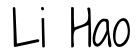
\includegraphics[width=.15\textwidth]{02-figures/signature.png} \par
\end{flushleft}

%%%%%%%%%%%%%%%%%%%%%%%%%%%%%%%%%%%%%%%%%%
\editorsection
%%%%%%%%%%%%%%%%%%%%%%%%%%%%%%%%%%%%%%%%%%

%%%%%%%%%%%%%%%%%%%%%%%%%%%%%%%%%
\point{Thank you for considering my and the reviewers’ comments, and resubmitting an improved version of the manuscript. However, I think you still need to clarify the use of some terms and the methodological approach, and to improve the discussion (please see the comments of the two reviewers). Particularly, I invite you to carefully consider the comments of the first reviewer about the uncertainty affecting your dataset and data availability. In addition, please see the following comments (lines refer to the manuscript without track changes).}
\reply{We thank the editor and the encouraging assessment of our revised study. In this round of revision, we have added the terms' definiation in Introduction, clarified the used method in Data and Methods, discussed the uncertainties in LAI, and incorporated your suggestions into the revised manuscript. In addition, we have made the python scripts available through an open code repository based on the comments from Dr. Florian Ulrich Jehn (\url{https://github.ugent.be/haohaoli/HESS-2022-Water-Yield.git}).}

%%%%%%%%%%%%%%%%%%%%%%%%%%%%%%%%%%%%%
\point{Introduction: the terms, climate, cryosphere and vegetation, have not been clarified. Please explain them.}
\reply{We thank Dr. Giulia Zuecco for pointing this out. In the revised manuscript, we define these key terms in the last paragraph in Introduction, which  helps readers understand this study clearly.}

\revised{51--54}{And then, we use DMC method to estimate the effects of climate that is indicated by effective precipitation (P-E, eP), vegetation (represented by Leaf Area Index, LAI), and cryosphere (e.g. melt waters from glaciers and snow) on magnitude and direction changes in WY (See Data and Methods).}

\nextreply{In addition, we have rephrased the Introduction part to avoid introducing these terms when we introduce other relevant studies. For example,}

\revised{26--27}{Therefore, comprehensively assessing long-term changes of WY, particularly magnitude and direction, is of great importance for the sustainable development of water resources in the  QTP \citep{yao2019recent}.}

\revised{29--30}{In recent years, WY has been significantly affected by multiply factors in the QTP.}

\revised{45--48}{Lastly, the present inadequate understanding of hydrological responses to complex interactions among multi-spheres limits the application of hydrological models in these mountainous watersheds \citep{pellicciotti2012challenges}.}

%%%%%%%%%%%%%%%%%%%%%%%%
\point{L83-85: Please report the exact GLEAM products and GLEAM version that were used for the data collection and analysis. Furthermore, please check the use of the term "evaporation" because in the supplementary material you used "evapotranspiration" (caption of Fig. S1).} 
\reply{Thank you for pointing this out. We have reported the version of the GLEAM used in our study. Also, we always keep "evaporation" or "E" in the revised version.}

\revised{84--85}{The evaporation (E) with a 0.25$^{\circ}$ spatial resolution is acquired from Global Land Evaporation Amsterdam Model (GLEAM) \textbf{version 3.5a}.} 

%%%%%%%%%%%%%%%%%%%%%%%%
\point{Table 1: Unclear use of the terms "glaciers and snow percentage".}
\reply{We thank the editor for pointing this out. We have added the column "area" to indicate the actual area of glaciers and snow, and another column "percent" to show its percentage of total area in individual basins.}

\begin{table}[hb]
  \centering
  \caption{Information of six basins divided by the locations of hydrological stations. The column "Tp" indicates the turning point using the Pettitt method, in which a significant turning point is labeled with *. Glaciers and snow is acquired from the land use and cover in 2000 (see Data). The unit of area is km$^2$, and the unit of elevation is m.}
  \label{tab:my-table}
  \begin{tabular}{cccccccl}
  \hline
  \multirow{2}{*}{Abbreviation} &
    \multirow{2}{*}{Full names} &
    \multirow{2}{*}{Station} &
    \multirow{2}{*}{\begin{tabular}[c]{@{}c@{}}Total \\ area \end{tabular}} &
    \multirow{2}{*}{\begin{tabular}[c]{@{}c@{}}Mean \\ elevation\end{tabular}} &
    \multicolumn{2}{c}{Glaciers and snow} &
    \multicolumn{1}{c}{\multirow{2}{*}{\begin{tabular}[c]{@{}c@{}}Tp\end{tabular}}} \\ \cline{6-7}
       &               &          &        &      & area & \multicolumn{1}{c}{percent} & \multicolumn{1}{c}{} \\ \hline
  HYZR & Headstream    & Lhatse   & 49,739 & 5,061 & 853        & 1.71                                & 1995                 \\
  UYZR & Upstream      & Nugesha  & 43,916 & 4,985 & 175        & 0.40                                & 1998*                \\
  NCR  & Nianchu River & Shigatse & 14,359 & 4,733 & 282        & 1.96                                & 1997*                \\
  MYZR & Midstream     & Yangcun  & 20,004 & 4,681 & 360        & 1.80                                & 1997*                \\
  LSR  & Lhasa River   & Lhasa    & 25,601 & 4,879 & 185        & 0.72                                & 1996                 \\
  LYZR & Downstream    & Nuxia    & 38,419 & 4,586 & 963        & 2.51                                & 1997                 \\ \hline
  \end{tabular}
\end{table}

\point{I think you should keep glacier and snow covers separated. For instance, you could quantify the glacier cover during the ablation season, and clearly describe in the text when the seasonal snowpack (outside the glacierized area) is present and at which elevations.}

\reply{Thanks for your suggestions. We agree that separating the effects of glaciers and snow melt is interesting. However, it is not trivial using the statistical techniques employed in this study. We use a statistical method (DMC) to isolate the effects of climate and vegetation on water yield. The remaining part from total water yield deviations is regarded as the contributions from cryosphere changes, which includes both changes in glacier and seasonal snow melt.}

\nextreply{In this study, we present the total area and percentage of glaciers and snow from the land use cover map in 2000 (Figure \ref{figS:lucc} and Table \ref{tab:my-table}), which supports the truth that the UBR basin is covered by glaciers and snow \citep{bibi2018climatic}. Hence, under global warming, this region is experiencing significant changes in cryosphere and having impacts on mountainous water resources, which fuels my interest in detecting hydrological changes and their causes.}

%%%%%%%%%%%%%%%%%%%%%%%
\point{Section 2.3.2: Please explain all subscripts used for WY. For equation 1, please describe the values that tp can take and check WYo(t), which is reported twice (based on the text above, I think it is not correct). The description for computing WYc and WYv is unclear; please rephrase and report the equations. Please always use capital (or small) letters for tp throughout the manuscript.}
\reply{Thank you for pointing them out. We hope to provide a general framework for six basins by using equations and relevant statements, so we always use "Tp" to indicate the turning point. Also, we have made sure that the term $WY_o(t)$ represents water yield from observations in the texts and equations. To state these equations clearly in the revised version, we firstly define a variable $\overline{WY_{ob}}$ that depicts the averaged water yield before Tp, which will reduce the numbers of variables within equations. And then, we add the range of Tp in equations, e.g. $t=Tp+1, Tp+2, \ldots, 2013$.}

\revised{125--126}{First, the averaged WY before Tp ($\overline{WY_{ob}}$, horizontal black line in Figure \ref{fig:example_DMC}b) is defined as:
\begin{equation}
    \overline{WY_{ob}} = \frac{\sum_{t=1982}^{t=Tp}WY_o(t)} {Tp-1982+1}
\end{equation}}

\revised{127--129}{Next, the total WY deviation ($\Delta WY_s(t)$, black diamond in Figure \ref{fig:example_DMC}c) can be calculated as the difference between WY observations after Tp ($WY_o(t)$, red point in Figure \ref{fig:example_DMC}b) and the averaged WY before Tp ($\overline{WY_{ob}}$), as follows:
\begin{equation} 
    \Delta WY_s(t)=WY_o(t)-\overline{WY_{ob}}, \ \  t=Tp+1, Tp+2, \ldots, 2013
\end{equation}}

\nextreply{We apologize for not describing $WY_c(t)$ and $WY_v(t)$ clearly, and we thank the editor for pointing this out. Here, $WY_c(t)$ ($WY_v(t)$) is calculated by using the cumulative eP (LAI) values after the Tp as input into the linear regression that is built based on the cumulative data of WY and eP (LAI) before Tp. We have rephrased this description in main text.}

\nextreply{Finally, we have rephrased these equations and related descriptions to match the six basins with different turning points, including (1) keeping "Tp" in the entire text and equations, and (2) giving the value of Tp in an example (\ref{fig:example_DMC}).}

%%%%%%%%%%%%%%%%%%%%%%%
\point{Section 4.2: Uncertainty in LAI has not been discussed. Furthermore, you should try to determine the sensitivity of your results to uncertain input data (in precipitation, evapotranspiration and LAI).}
\reply{Thanks for your suggestions. We have added a discussion on the uncertainties of GIMMS LAI used in the revised manuscript.}

\revised{264--268}{GIMMS LAI has the advantage of capturing ecosystem structure, and thus is widely used to assess vegetation conditions and their effects on hydrological changes \citep{zhu2016greening,forzieri2020increased,gonsamo2021greening}. While, LAI ignores vegetation's physiology process \citep{fang2019overview}; \citet{hu2022decoupling} indicates that LAI can cope with hydro-climatic fluctuations in arid environments, while the tradeoff between ecosystem structure (LAI) and physiology (photosynthesis per unit leaf area) becomes stronger in humid climates. Thus, using LAI products in energy-limited regions may result in biased assessments of vegetation effects on water yield.}

\nextreply{Thanks for your suggestions about the uncertainties. We acknowledge that it is very important to use multi-source climate and vegetation data. This can provide a clear visualization about uncertainties among datasets and associated results. However, our study here focuses on a vast and mountainous watershed, where the observation networks and related datasets are limited and also are extremely difficult to acquire. In addition, popular climate data, e.g. MSWEP, ERA5, CRU, do not perform well in such complex environments and limited ground observations \citep{sun2020precipitation}. To overcome this, we collected the long-term annual runoff observations to indicate water yield changes. And, the high-resolution precipitation data is developed for depicting spatial and temporal precipitation changes in the Yarlung Zangbo River basin (UBR basin in this study) by \citealt{sun2020precipitation}. Hence, the dataset about precipitation may be the best for the UBR basin, to our knowledge. For evaporation, GLEAM dataset has been widely validated across world, and particularly in various hydroclimates in China. There are some uncertainties among different LAI datasets due to input data, retrieval algorithms and the vegetation characterization, but GIMMS LAI3g is used in this study according to previous studies that have analyzed the effects of vegetation greenness on water yield pattern \citep{zhu2016greening, forzieri2020increased, gonsamo2021greening}. Thus, this study provides the essential information for water resource management in the UBR basin that received less attention before based on the multi-station runoff observations and climate gridded data.}

\point{L272-275: Based on Fig. S8, I do not clearly see the "peak water". Please revise the text and/or the figure to support your statement.}
\reply{Thanks for your questions. We here discuss our results and "peak water" using the framework (\url{https://www.nature.com/articles/s41558-017-0049-x/figures/1}, \citealp*{huss2018global}) according to the second reviewer in the first round of review. Also, we provide the reasons to support our statement in the revised manuscript.}

\revised{283--286}{In addition, in the headwaters, WY resulting from the cryosphere continues to increase with temperature until a maximum is reached, beyond which cryospheric contribution to total WY begins to decrease (Figure \ref{figS:warming-and-cryosphere}a), which may show that the melt waters from glaciers have already surpassed the "peak water". The hydrological changes will substantially affect future water resources management, and thus the projections of the occurrence time of "peak water" will be important in managing mountainous water resources.}

\point{Figure S3: Please explain what the error bars indicate.}
\reply{Thanks for your comments. We have revised the definitions of the error bars for Figure \ref{figS:P-and-WY}.}

\begin{figure*}[ht]
  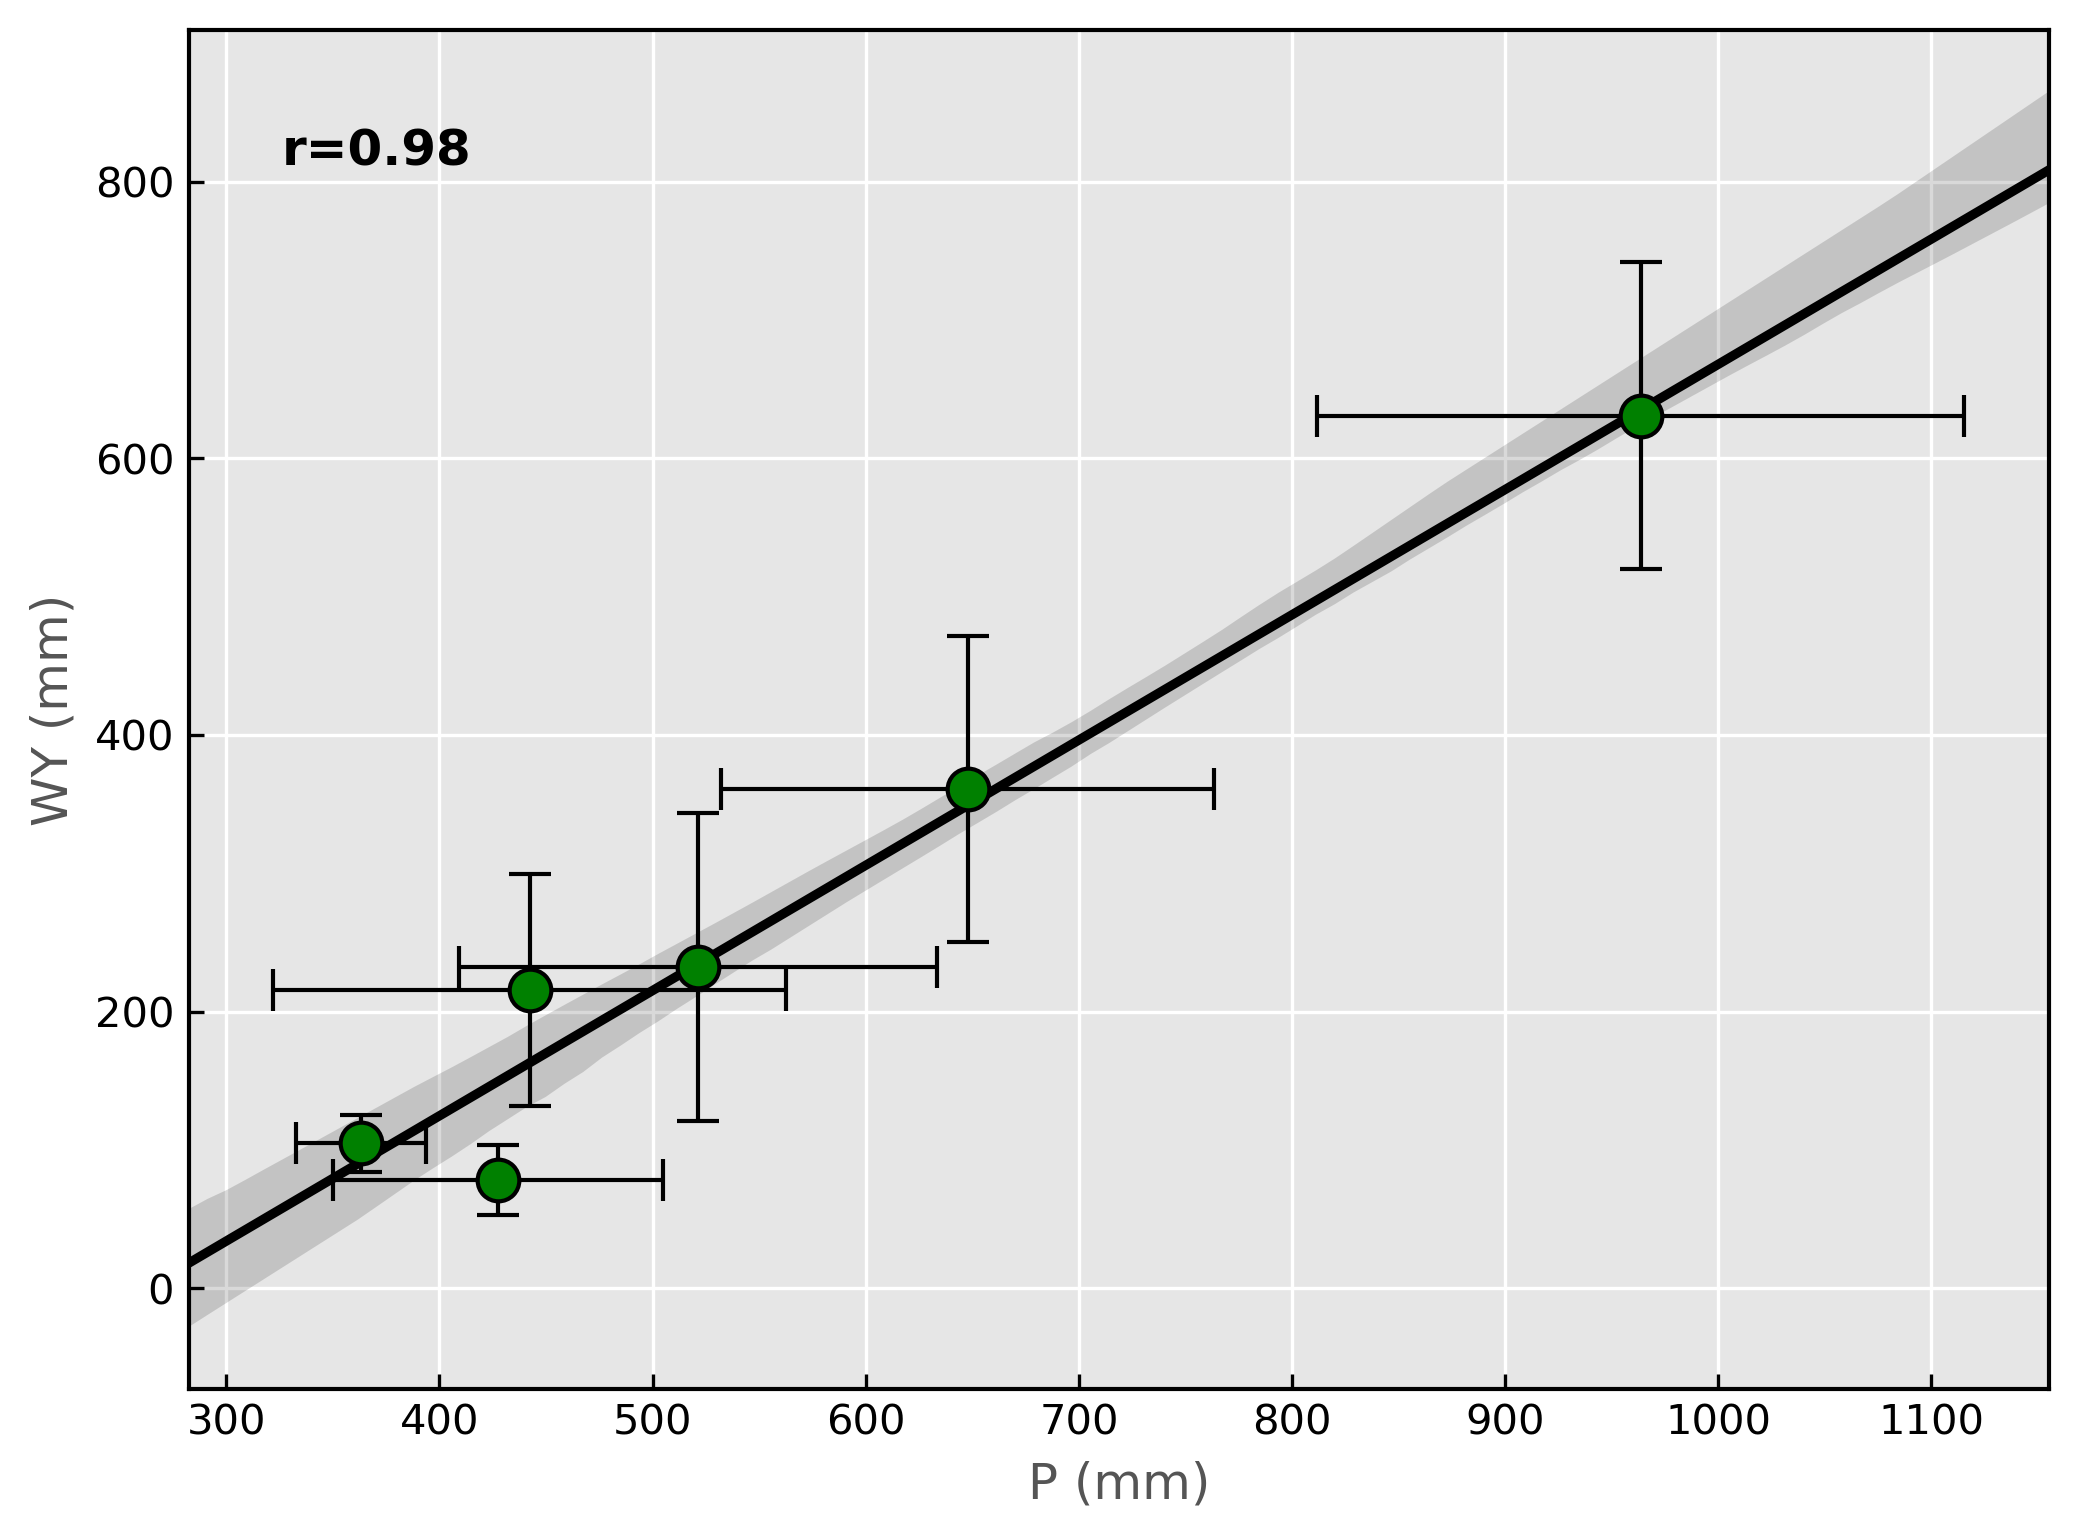
\includegraphics[width=12cm]{02-figures/pre-and-water-yield.png}
  \captionsetup{labelformat=empty}
  \caption{Figure \ref{figS:P-and-WY}. The relationship between precipitation (P) and water yield
  (WY) in the entire UBR basin.
  \textbf{The error bar represents one standard deviation of P (x-axis) and WY (y-axis)}. 
  The shading area indicates the 95\% confidence interval of the fitting.}
\end{figure*}

\bibliographystyle{copernicus}
\bibliography{reference.bib}

%%%%%%%%%%%%%%%%%%%%%%%%%%%%%%%%%%%%%%%%%%
\reviewersection % reviewer 01
%%%%%%%%%%%%%%%%%%%%%%%%%%%%%%%%%%%%%%%%%%
\sect{Main Comments}

\point{I appreciate the effort that authors put into revising their manuscript and I think it has improved considerably. However, I still have some problems with it. This is mainly concerned with your data and statistics. For example you are writing: "However, with the help of the Second Tibetan Plateau Scientific Expedition and Research, the observation networks in meteorology, cryosphere and hydrology will be built, which is expected to benefit reliable precipitation and evaporation estimation, and make developing physically-based cryosphere-hydrological modeling possible". This sounds to me like you cannot really estimate your uncertainty right now and it is unclear if your analysis would give you the same results if you could rerun your analysis with better data.}
\reply{Thanks for your comments. Our study focuses on several watersheds in the UBR basin and investigate the hydrological changes and potential causes based on observed runoff data and new precipitation product developed for this region. While, the study scale in space and time may ignore some important process that are much more significant in smaller scales. Thus, we expect that more observation networks and experimental datasets in the field scale will help us understand the physical mechanisms of the hydrological cycle in this region. We made some revisions as following:}

\revised{271--274}{With the help of the Second Tibetan Plateau Scientific Expedition and Research, the observation networks in meteorology, cryosphere and hydrology will be built, which is expected to better understand hydrological process in this region, and make developing physically-based cryosphere-hydrological modeling possible \citep{wang2022observing}.}

\point{Still, this not really your fault that better data does not exist (yet?), so it seems like your analysis is the best you could do given the current data constrains. This should also be emphasized in the paper.}
\reply{Thanks for your understanding. To my knowledge, this study uses the multi-station observed runoff and new precipitation product designed for the UBR basin, and thus provides some important information that previous studies did not reveal. We have emphasized it in main text.}

\point{In addition, this makes it much more important that your work is reproducible, which it is not at the moment. Neither the code nor the data is openly available. This means even if better data becomes available your results still cannot be verified. Therefore, to make this paper a valuable contribution I think it is important that a documented and citable repository exists for the code (preferably as Jupyter Notebooks) and if possible, the data as well.}
\reply{We agree with the reviewer. Reproducibility is ensured through GitHub. We have provided a link for accessing the Jupyter Notebook via the git repository (\url{https://github.ugent.be/haohaoli/HESS-2022-Water-Yield.git}). However, runoff observations can't be shared due to a confidentiality contract.}

\point{I also think you misunderstood my comment 1.14. With "corrected" my question was if you account for doing multiple statistical tests in a row (\url{https://en.wikipedia.org/wiki/Multiple_comparisons_problem}). If not you have to do a correction (e.g. \url{https://en.wikipedia.org/wiki/Bonferroni_correction}).}
\reply{Thanks for pointing it out. We use the Bonferroni method to correct p values that still support the main results, and report the method and relevant descriptions using the corrected p values in the revised manuscript. But, the change from the significant to non-significant correlation using the corrected p values is observed in the relationship between vegetation contributions and total water yield changes in the UYZR basin (see the updated Figure \ref{fig:attribution-direction}b).}

\revised{151--152}{The Student's t-test with the Bonferroni correction \citep{bonferroni1935calcolo} is used to detect the statistical significance of the correlation coefficient at the level of 0.05.}

\sect{Minor comments}

\point{The figure caption of Figure 2 isn't really that helpful. First, this is an example and not a schema. Secondly, It does not really "show" me how the effects are estimated. This would need additional explanations in the figure and the caption to become a schema.}
\reply{Thanks for your questions. We describe the DMC used in this study by (1) providing a general framework using equations and relevant statements, and (2) giving an example to help describe the framework. Thus, in the revised version, we have rephrased the \textbf{equations} and \textbf{related descriptions} to show how to estimate the effects, while the Figure \ref{fig:example_DMC} gives an \textbf{example} to help us better describe these equations, where we give the value of the turning point in the caption.}

\point{Line 180-183: How can they be additive and offsetting at the same time?}
\reply{Thanks for your question. The additive or offsetting effects are seen in \textbf{different basins} (Figure \ref{fig:attribution-magnitude}); for example, the additive effect is observed in MYZR basin, while the offsetting effect is found in HYZR basin. Also, we revised the statement in the main text.}

\revised{182--184}{Climate and cryosphere -- two important factors affecting WY -- together contribute to over 80\% average magnitude increases of WY in the entire UBR basin; however, they play both additive or offsetting roles \textbf{in different basins} (Figure \ref{fig:attribution-magnitude}) ... }

%%%%%%%%%%%%%%%%%%%%%%%%%%%%%%%%%%%%%%%%%%
\reviewersection % reviewer 02
%%%%%%%%%%%%%%%%%%%%%%%%%%%%%%%%%%%%%%%%%%
\point{The study of Li et al. is about the analysis of long -term water yield from the Upper Brahmaputra River basin associated with potential drivers such as climate, vegetation, and the cryosphere. Based on hydro-climatic data, the authors identify turnings points to infer major water yield shifts in the basins. Furthermore, the study reports that climate may act as driver for downstream water yield while meltwaters control water yield further upstream. It is also found that melt water dynamics balance out low flow conditions induced by climate. The insights gained in this study may help to better understand large scale drivers of water yield and improve water management strategies. Besides, only minor comments regard typing errors and the language quality (see specific comments below). The manuscript generally is of good English.}

\reply{We thank the reviewer for the constructive comments. We revised some typos in the revised version and gave a point-to-point response below.}

\sect{Specific comments}

\point{p. 1, l. 4: Please modify ‘find that’}
\reply{Thanks. We have revised this.}

\point{p. 1, l. 5: At this stage the reader will not understand the upstream and downstream direction of water yield while it becomes clearer after reading the entire manuscript. I recommend mentioning instead only controls of water yield in the upper and lower reaches.}
\reply{Thanks. We now realized that the description may confuse readers, and thus we revised the related descriptions. }
\revised{5--6}{... magnitude increases in WY range from $\sim$10\% to $\sim$80\%, while its directions reverse from \textbf{the increase} to \textbf{decrease} after the late 1990s.}

\point{p. 1, l. 14: It would be great to define water yield in this section, simply saying that it is based on the total runoff of a basin.}
\reply{Thanks. We have used "runoff depth" to further explain "water yield" in the beginning of the introduction.}

\revised{14--15}{Water yield (or runoff depth, WY) in mountainous watersheds is crucial for sustaining fragile ecosystems in headwaters ... }

\point{p. 2, l. 48: Please rephrase this sentence.}
\reply{Thanks, we have rewritten this statement.}
\revised{48--49}{While, long-term observed runoff records and recent high-resolution precipitation data in the UBR basin provide a valuable opportunity to estimate runoff responses to warming by statistical methods.}

\point{p. 5, l. 85: showed instead of shown}
\reply{Thanks, we have revised that.}
\revised{85}{GLEAM evaporation has been validated in different biome types in China and \textbf{showed} high correlations with in-situ eddy covariance E \citep{yang2017multi}.}

\point{p. 5, l. 100: In this line, you should add further explanation on turning points, their definitions and shortly how the Pettitt method works.}
\reply{Thanks for your suggestions. We have added the advantages of the Pettitt method.}
\revised{101--102}{The Pettitt method has the advantages of the non-parametric, rank-based and distribution-free for finding the abrupt variation in a time series.}

\point{p. 5, l. 106: The fact that the cryosphere represents meltwaters from snow and ice should appear earlier in the text.}
\reply{Thanks. We have provided some descriptions in the last paragraph in Introduction.}

\revised{52--55}{And then, we use DMC method to estimate the effects of climate (effective precipitation, P-E, eP), vegetation (Leaf Area Index, LAI), and cryosphere (e.g. melt waters from glaciers and snow) on magnitude and direction changes in WY (See Data and Methods).}

\point{p. 8, l. 158: The first sentence is redundant to what is said earlier in the methods.}
\reply{Thanks, we have deleted this sentence.}

\point{p. 9, l. 168: becomes instead of become}
\reply{Thanks, we have revised the typo.}
\revised{170--171}{... we find that \textbf{the trend} \textbf{is} positive before Tp, but \textbf{becomes} negative afterward in most basins.}

\point{p. 11, l. 205: a word is missing as it seems. Maybe observation, result, or finding?}
\reply{I am sorry for that. We have replaced "The is ..." with "This is ..."}
\revised{206--207}{... and snow under continuous warming. \textbf{This is} further verified by the relationship of cryospheric contributions ...}

\point{p. 13, l. 225: controlling instead of control}
\reply{Thanks, we have revised the whole sentence.}
\revised{228--229}{Climate, especially precipitation, still \textbf{controls} the declining WY trend after ...}

\point{p. 13, l. 242-244: Please rephrase this sentence.}
\reply{Thanks for your comments. We have described the sentence clearly.}
\revised{245--247}{While, in some other mountainous basins, human activities, such as urbanization, dam regulation and irrigation, may consume severely water resources or change seasonal runoff patterns; \textbf{thus it is necessary to} consider anthropogenic impacts when assess river flow changes via the statistical models \textbf{in these regions}.}

\point{p. 13, l. 244: "on the one hand" is missing previously}
\reply{ Thanks. "In addition" may be better to link these sentences. }

\point{p. 13, l. 245: Please add further details on the nonlinear processes you are referring to here.}
\reply{Thanks. We have added some examples into the main text.}
\revised{248--250}{... some nonlinear process among water, vegetation and cryospheric melting. For example, the role of vegetation in hydrological process is expected to be complex due to biophysical (e.g., via transpiration and albedo changes) and biochemical (e.g., via CO2 uptake and release) feedbacks (\citealtrev{bonan2008forests,krich2022decoupling}).}

\point{p. 13, l. 246: ‘interactions of’}
\reply{Thanks. We have rephrased this sentence.}

\point{p. 14, l. 251: remove ‘while’}
\reply{We have removed "while".}

\point{p. 15, l. 283: remove ‘with’}
\reply{We have removed "with".}

\point{Table 1: Correct ‘turning point’.}
\reply{Thanks for your comments. We have kept the abbreviation "Tp" of "turning point" in the revised manuscript.}

\point{Figure 4: Labels are too small, please enlarge for better visibility.}
\reply{Thanks. We have adjusted the font size for all figures in main text and supplementary.}

\point{Figure S8: It is highly questionable why, for some data clouds (subplot b,d,f), the polynomial fitting was used. Generally, the best fit among several methods is reported, except there is an important reason for a specific method to give.}
\reply{Thanks for your questions. We tried to link our results with present findings, e.g. "peak water" according to the second reviewer in the first round of review. Hence, we referred to this framework (\url{https://www.nature.com/articles/s41558-017-0049-x/figures/1}, \citealprev*{huss2018global}) that shows the response of runoff from a glacierized basin to continuous atmospheric warming (years). Hence, we used the polynomial curve to depict relationship between the cryospheric contribution (this study) and the air temperature. Indeed, we can see the clear pattern in headwaters that cryospheric contribution increases firstly and decrease later with temperatures, which may imply the "peak water" as shown in \citeprev{huss2018global}. Honestly, we acknowledge that the simple statistical methods, e.g. polynomial curve, may be not the best way to describe the relationship between cryospheric contribution (y-axis) and air temperature (x-axis) or revealing the "peak water". Thus, we keep cautions about the explanation, and only report that the HYZR basin may have surpassed the "peak water" in the revised text.}

\bibliographystylerev{copernicus}
\bibliographyrev{reference.bib}

\end{document}